In questo capitolo vengono spiegati i vari metodi di ottimizzazione utilizzati poi negli ensemble.

\section{Metodo Adam}
Adam (Adaptive momentum estimation) è un metodo di ottimizzazione introdotto in [citazione] che calcola il learning rate adattivo per ciascun parametro combinando i concetti di momento e di gradiente adattivo. La regola di aggiornamento si basa sul valore del gradiente al tempo $t$ e sulle medie mobili del gradiente e del suo quadrato. Più precisamente, il metodo Adam definisce le due medie mobili esponenziali (Exponential Moving Average, EMA) $m_{t}$ (primo momento) e $u_{t}$ (secondo momento) come:
\begin{equation}
	m_{t} = \rho_{1}m_{t-1}+(1-\rho_{1})g_{t}
\end{equation}
\begin{equation}
	u_{t} = \rho_{2}u_{t-1}+(1-\rho_{2})g_{t}^{2}
\end{equation}
dove $g_{t}$ è il gradiente al tempo $t$, $g_{t}^{2}$ è il quadrato del gradiente nei termini del quadrato delle sue componenti, $\rho_{1}$ e $\rho_{2}$ sono iper-parametri che rappresentano il tasso di decadimento esponenziale per il primo momento e per il secondo (solitamente settati a 0.9 e 0.999, rispettivamente); inizialmente i momenti sono inizializzati a 0: $m_{t} = u_{t} = 0$. 

Siccome i valori delle due medie mobili potrebbero essere molto piccoli a causa della loro inizializzazione a zero, soprattutto nei primi steps, gli autori del metodo Adam hanno proposto una nuova versione che presenta una correzione ai due momenti:
\begin{equation}
	\hat{m_{t}} = \frac{m_{t}}{(1-\rho_{1}^{t})}
\end{equation}

\begin{equation}
	\hat{u_{t}} = \frac{u_{t}}{(1-\rho_{2}^{t})}
\end{equation}


Infine l'ultimo aggiornamento per ogni parametro $\theta_{t}$ della rete è:

\begin{equation}
	\theta_{t} = \theta_{t-1}-\lambda\frac{\hat{m_{t}}}{\sqrt{\hat{u_{t}}}+\epsilon}
\end{equation}

dove $\lambda$ è il learning rate, $\epsilon$ è un numero positivo molto piccolo in modo tale da prevenire una possibile divisione per 0 (solitamente $\epsilon=10^{-8}$).

\section{Metodo diffGrad}
diffGrad è un metodo di ottimizzazione introdotto in (citazione) che tiene conto della differenza del gradiente per regolare il learning rate.

Si può osservare che quando i cambiamenti del gradiente si riducono durante l'addestramento allora ciò è spesso indicativo della presenza di minimi globali, diffGrad applica una regolazione adattiva data dalla differenza tra il gradiente al tempo $t$ e quello immediatamente passato $t-1$ in modo tale da impostare i parametri nel minimo globale. Pertanto la dimensione del learning rate sarà alta per modifiche repentine del gradiente e bassa per modifiche più lente e graduali.

Per poter definire la regola di aggiornamento occorre determinare il valore assoluto della differenza del gradiente in due istanti di tempo consecutivi:
\begin{equation}
	\Delta g_{t} = |g_{t-1}-g_{t}|
\end{equation}

Infine l'ultimo aggiornamento da effettuare per ogni parametro $\theta_{t}$ della rete è simile all'equazione [5.5], dove $\hat{m_{t}}$, $\hat{u_{t}}$ sono definite come in [5.3], e [5.4] e il learning rate è modulato dalla sigmoide di $\Delta g_{t}$:
\begin{equation}
	\xi_{t} = Sig(\Delta g_{t})
\end{equation}
\begin{equation}
	\theta_{t+1} = \theta_{t}-\lambda\cdot\xi_{t}\frac{\hat{m_{t}}}{\sqrt{\hat{u_{t}}}+\epsilon}
\end{equation}
 
\section{Nuovi metodi di ottimizzazione}
Vengono proposte di seguito diverse varianti del metodo di ottimizzazione diffGrad e Adam:
\begin{itemize}
	\item DGrad si basa sulla media mobile dei quadrati dei parametri del gradiente componente per componente;
	\item Cos\#1 è una variante di DGrad basata sull'applicazione di un cyclic learning rate (CLR);
	\item Exp si basa sull'applicazione di una funzione esponenziale;
	\item Sto è un approccio stocastico per settare il learning rate, che ha lo scopo di evitare che l'ottimizzatore vada in stallo in caso di una zona piatta (plateau).
\end{itemize}
Le varianti proposte differiscono nella definizione del parametro $\xi_{t}$, mentre ciascuna utilizza l'equazione [5.8] nell'aggiornamento finale dei parametri $\theta_{t}$. 

\textbf{DGrad} riprende le idee di diffGrad ri-definendo il valore assoluto della differenza del gradiente in due istanti di tempo consecutivi:
\begin{equation}
	\Delta ag_{t} = | g_{t}-avg_{t} | 
\end{equation}
dove $avg_{t}$ è la media mobile del quadrato, componente per componente, dei parametri del gradiente; poi normalizziamo $\Delta ag_{t}$ con il suo massimo e otteniamo:
\begin{equation}
	\Delta\hat{ag_{t}} = \left(\frac{\Delta ag_{t}}{max(\Delta ag_{t})} \right)
\end{equation}
e definiamo $\xi_{t}$ come:
\begin{equation}
	\xi_{t} = Sig(4 \cdot \Delta \hat{ag_{t}})
\end{equation}
dove il fondamento logico che porta a moltiplicare per "4" l'argomento della funzione sigmoidea è aumentare l'intervallo di output della funzione stessa.

\textbf{Cos\#1} è una variante di DGrad che sfrutta l'idea di utilizzare un learning rate ciclico, con l'obiettivo di migliorare l'accuratezza della classificazione senza tuning e con meno iterazioni [citazione].
Occorre utilizzare una funzione periodica per definire l'intervallo di variazione del learning rate. In questo caso è stata utilizzata la funzione coseno $\cos()$, definita come segue:
\begin{equation}
	lr_{t} = \left(2-\left\lvert\cos\left(\frac{\pi \cdot t}{steps}\right)\right\rvert e^{-0.01 \cdot (mod(t,steps)+1)}\right)
\end{equation}
dove la funzione $mod()$ denota la funzione modulo e il periodo è definito da $steps=30$.

\vspace{0.25cm} 
\begin{center}
	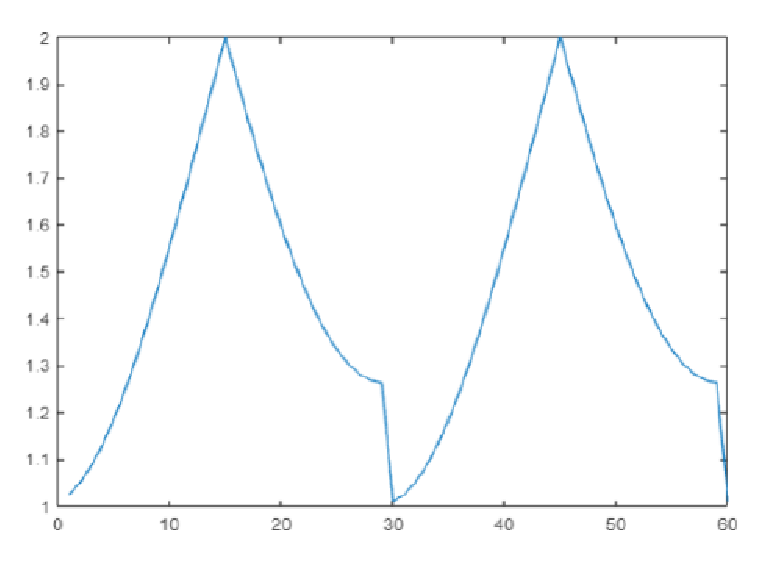
\includegraphics[scale=0.5]{images/clr.eps} %correggere GRU(H UNITA' nascoste)
	\captionof{figure}{Cyclic learning rate}
	\label{Figura 1.}
\end{center}
\vspace{0.25cm}

In questa variante $lr_{t}$ è utilizzato come fattore moltiplicativo di $\hat{ag_{t}}$ nella definizione di $\xi_{t}$, che diventa:
\begin{equation}
	\xi_{t} = Sig(4 \cdot lr_{t} \cdot \Delta \hat{ag_{t}})
\end{equation}


\textbf{Exp} consiste in due semplici operazioni quali prodotto ed esponenziale. Lo scopo di questa variante è di limitare l'effetto di grandi variazioni del gradiente, ma anche di consentire alla funzione di convergere per piccoli valori. L'equazione (18) ha un andamento che decade più lentamente dell'esponenziale negativo per alti valori e, grazie alla normalizzazione, dà meno attenzione alle variazioni del gradiente che tendono a zero, aumentando l'area di maggior guadagno:
\begin{equation}
	lr_{t} = \Delta ag_{t} \cdot e^{-2\cdot\Delta ag_{t}}
\end{equation}

Il parametro $\xi_{t}$ è dato dalla normalizzazione del precedente learning rate per il suo massimo, moltiplicato per "1.5", che aiuta a spostare la media verso l'unità.
\begin{equation}
	\xi_{t} = 1.5 \cdot \frac{lr_{t}}{\max(lr_{t})}
\end{equation}

\vspace{0.25cm} 
\begin{center}
	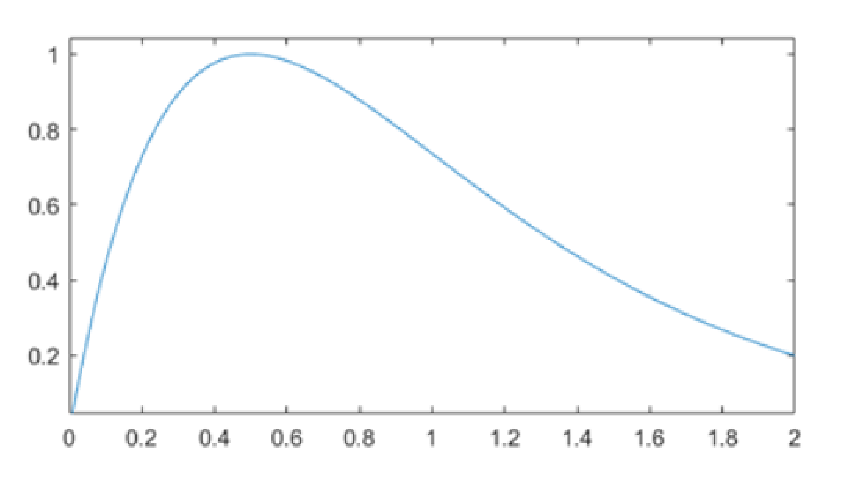
\includegraphics[scale=0.5]{images/exp.eps} %correggere GRU(H UNITA' nascoste)
	\captionof{figure}{Plot dell'eq. 5.14}
	\label{Figura 1.}
\end{center}
\vspace{0.25cm}


\textbf{Sto} è una variante progettata per ridurre la possibilità che l'ottimizzatore possa andare in stallo su zone piatte aggiungendo rumore gaussiano bianco additivo (Additive White Gaussian Noise, AWGN) al learning rate. Il rumore additivo è indipendente dalla direzione del gradiente, quindi aggiunge un certo grado di incertezza alla ricerca dell'ottimo e potrebbe aiutare a trovare il minimo locale quando l'ottimizzatore fa fatica a causa di un learning rate troppo grande.

Sia $X$ una matrice di variabili casuali uniformi e indipendenti nell'intervallo $[0,1]$ e $J$ una matrice di tutti "1":
\begin{eqnarray*}
	\mathcal{X} =
	\begin{bmatrix}
		X_{1,1} & \cdots & X_{1,n}\\
		\vdots & \ddots & \vdots\\
		X_{m,1} & \cdots & X_{m,n}
	\end{bmatrix}
	\hspace{45pt}
	J = 
	\begin{bmatrix}
		1 & \cdots & 1\\
		\vdots & \ddots & \vdots\\
		1 & \cdots & 1
	\end{bmatrix}
\end{eqnarray*}
dove $X_{i,j} \sim \mathcal{U}(0,1)$ sono variabili casuali con funzione di densità di probabilità uniforme. Il learning rate è definito come:

\begin{equation}
	lr_{t} = \Delta ag_{t} \cdot e^{(-4\cdot\Delta ag_{t})} \cdot (\mathcal{X} + 0.5 \cdot J)
\end{equation}
dunque
\begin{equation}
	\xi_{t} = 1.5 \cdot \frac{lr_{t}}{\max(lr_{t})}
\end{equation}

Nell'eq. 20 la matrice $J$ viene utilizzata per shiftare l'intervallo di $X$ di 0.5 per spostare la media su 1.
